[130 v\textsuperscript{o}] et lignes imaginables: il est manifeste, que tous les coups que ces deux corps\protect\index{Sachverzeichnis}{corps} re\c{c}oivent des vagues \edtext{de la liqueur\protect\index{Sachverzeichnis}{liqueur}}{\lemma{}\Afootnote{de la liqueur\protect\index{Sachverzeichnis}{liqueur} \textit{ erg.} \textit{ L}}}, contribuent \`{a} la conservation de leur contiguit\'{e} contre une separation directe. Puisque tous les coups donnent contre les superficies exterieures, lesquelles estant oppos\'{e}es l'une \`{a} l'autre font les corps\protect\index{Sachverzeichnis}{corps} estre pressez l'un vers l'autre, car tous les coups que le corps\protect\index{Sachverzeichnis}{corps} \textit{AB} peut recevoir viennent de \textit{E} vers \textit{F} et tous ceux qui rencontrent le corps\protect\index{Sachverzeichnis}{corps} \textit{CD} viennent de \textit{F} vers \textit{E}.\pend 
\clearpage
%Zeitz auskommentiert\begin{center}                    
%                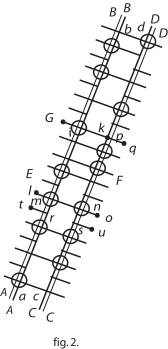
\includegraphics[width=0.38\textwidth]{images/37_3_130v}\\\textit{[Fig. 3]}
%                        %\caption{Bildbeschreibung}
%                        \end{center} 
                        \pstart Voila la substance de cette Hypothese. \textso{L'objection} est que cela seroit veritable, si les corps\protect\index{Sachverzeichnis}{corps} \textit{AB} et \textit{CD} estoient sans pores: Mais comme ceux même qui introduisent cette matiere subtile\protect\index{Sachverzeichnis}{mati\`{e}re!subtile} luy font passage par les corps\protect\index{Sachverzeichnis}{corps!solide} les plus solides, il s'ensuit que les superficies interieures des corps\protect\index{Sachverzeichnis}{corps} contigus mais poreux, seront aussi frapp\'{e}es par le mouuement de la matiere. Car comme il paroist dans la 2\textsuperscript{me} figure
 toutes les lignes \edtext{du mouuement}{\lemma{}\Afootnote{du mouuement \textit{ erg.} \textit{ L}}} qui viennent du cost\'{e} de \textit{E} \edtext{comme \textit{gik} et \textit{lmno}}{\lemma{}\Afootnote{comme \textit{gik} et \textit{lmno} \textit{ erg.} \textit{ L}}} et passent par les pores du corps\protect\index{Sachverzeichnis}{corps} \textit{AB}\edtext{, si \textit{i} vel \textit{m} rencontrent}{\lemma{\textit{AB}}\Afootnote{ \textit{ (1) }\   \textbar\ heurtent \textit{ erg.}\ \textbar\  comme par exemple la ligne du coup \textit{gik}, qui passe par le pore \textit{i}, si elle rencontre \textit{ (2) }\ , si \textit{i} vel \textit{m} rencontrent \textit{ L}}} necessairement ou un autre pore dans le corps\protect\index{Sachverzeichnis}{corps} \textit{CD} comme \textit{lm} rencontre \textit{n}, en quel cas le coup de la vague passe \edtext{outre}{\lemma{}\Afootnote{outre \textit{ erg.} \textit{ L}}} sans s'arrester ou contribuer \`{a} l'union ou des-union des corps\protect\index{Sachverzeichnis}{corps}, ou \edtext{elles rencontrent}{\lemma{}\Afootnote{elles rencontrent \textit{ erg.} \textit{ L}}} la superficie interieure du corps\protect\index{Sachverzeichnis}{corps} oppos\'{e}e comme \textit{gi} donne contre \textit{k} et tous les coups de cette nature, dont il y a une infinit\'{e}, contribuent \`{a} la des-union des corps\protect\index{Sachverzeichnis}{corps}. \textso{La response} \`{a} cette objection \edtext{est telle: que les coups}{\lemma{objection}\Afootnote{ \textit{ (1) }\ que tous \textit{ (2) }\ est telle: que les coups \textit{ L}}} de cette nature qui heurtent les superficies interieures des corps\protect\index{Sachverzeichnis}{corps} \edtext{et qu'on pourroit appeller separatifs}{\lemma{et}\Afootnote{qu'on pourroit appeller separatifs \textit{ erg.} \textit{ L}}}, sont tous compensez par des autres coups \edtext{unitifs}{\lemma{}\Afootnote{unitifs \textit{ erg.} \textit{ L}}} qui frappent en même temps la superficie exterieure du même corps\protect\index{Sachverzeichnis}{corps} au même endroit, comme le coup \textit{gik} est compens\'{e} ou d\'{e}truit par le coup \textit{qp}. Mais qu'il y a des coups unitifs, ou contre les superficies exterieures, qui ne sont pas compensez.\pend \pstart  Car il y a trois cas possibles, tantost un pore d'un corps\protect\index{Sachverzeichnis}{corps} estant joint contre un pore de l'autre corps\protect\index{Sachverzeichnis}{corps}, comme \textit{m} contre \textit{n} o\`{u} les coups sont ny unitifs ny separatifs; tantost un pore estant joint contre une partie solide, comme \textit{i} contre \textit{k} o\`{u} l'un coups, du cost\'{e} du pore est separatif, l'autre du cost\'{e} de la partie \edtext{solide}{\lemma{}\Afootnote{solide \textit{ erg.} \textit{ L}}} est unitif; tantost une partie solide estant jointe contre une partie solide, comme \textit{r} contre \textit{s} o\`{u} les coups de deux costez \textit{tr} et \textit{us} sont unitifs, et par consequent ny compensez ny detruits par d'autres separatifs.\pend \pstart  On pourroit repartir \edtext{que}{\lemma{repartir}\Afootnote{ \textit{ (1) }\ qu'il peut avoir \textit{ (2) }\ que \textit{ L}}} les deux corps\protect\index{Sachverzeichnis}{corps}, ou pore est tousjours joint \`{a} pore, ou partie solide, seront sans union, item que \edtext{deux corps}{\lemma{que}\Afootnote{ \textit{ (1) }\ un corps\protect\index{Sachverzeichnis}{corps|textit} \textit{ (2) }\ deux corps \textit{ L}}} \edtext{bien joints par cette pression}{\lemma{corps}\Afootnote{ \textit{ (1) }\ qui ont est\'{e} pour \textit{ (2) }\ bien joints par cette pression \textit{ L}}} en glissant un peu changeront de connexion, \edtext{et perdront toute l'union, ou au moins une grande partie}{\lemma{connexion,}\Afootnote{ \textit{ (1) }\ et se separeront ou d'abord ou par une moindre force \textit{ (2) }\ et [...] partie \textit{ L}}}, si les parties \edtext{solides}{\lemma{}\Afootnote{solides \textit{ erg.} \textit{ L}}} ou toutes, ou pour la pluspart, qui estoient auparavant joinctes aux parties solides \edtext{du corps\protect\index{Sachverzeichnis}{corps} oppos\'{e}}{\lemma{}\Afootnote{du corps\protect\index{Sachverzeichnis}{corps} oppos\'{e} \textit{ erg.} \textit{ L}}} comment \`{a} present \edtext{rencontrer les pores}{\lemma{present}\Afootnote{ \textit{ (1) }\ repondre aux por \textit{ (2) }\ rencontrer les pores \textit{ L}}}.\pend \pstart  Mais \edtext{sans s'arrester la dessus}{\lemma{}\Afootnote{sans s'arrester la dessus \textit{ erg.} \textit{ L}}} il y a des \edtext{autres}{\lemma{}\Afootnote{autres \textit{ erg.} \textit{ L}}} Repliques bien plus